\documentclass[fullscreen=true, unicode, bookmarks=false]{beamer}
\usepackage[T2A]{fontenc}
\usepackage[utf8]{inputenc}
\usepackage[english, russian]{babel}
\usepackage{amsmath}
\usepackage{amsmath,amsfonts,amssymb}
\usepackage[export]{adjustbox}
\usepackage{textgreek}
\newtheorem{rustheorem}{Теорема }
\newtheorem{ruslemma}{Лемма }
\sloppy

\setbeamertemplate{navigation symbols}{}

\DeclareMathOperator{\arsh}{arsh}

\usetheme{Warsaw}

\usecolortheme{whale}

\usefonttheme{professionalfonts} % default family is serif

\setbeamertemplate{footline}{\hspace*{.5cm}\scriptsize{\insertshorttitle
\hspace*{50pt} \hfill\hspace*{.5cm}}\vspace{5pt}} 

\setbeamercolor{bibliography entry author}{fg=black}

\title[]{ {\huge Потеря устойчивости нулевого решения одного класса краевых задач со специальными краевыми условиями} }   
\author[]{{\Large Леонид Ивановский}} 
\date{ }
\institute[]

\begin{document}

\begin{frame}
\titlepage
\end{frame} 

\begin{frame}

$$
\dot{T} = T'',
$$
$$
T(0, t) \, = 0, \quad T'(1, t) \, = f(1 - T (x_0, t)) \sigma (1 - T (x_0, t)), 
$$

$$ t \geqslant 0, \quad x \in [0,1], \quad x_0 \in [0, 1), \quad  b > 0, \quad \alpha, \in \mathbb{R}. $$

\vfill

$$  f\equiv\left(1 - T\left(\frac{1}{2}, t \right)\right)^2. $$

\vfill

Rudyi A.S. Theoretical Fundamentals of the Method for Thermal Diffusivity Measurements from Auto-Oscillation Parameter in a System with a Thermal Feedback // International Journal of Thermophysics, Vol. 14, No. 1, 1993, pp. 159 --172.

\end{frame}

\begin{frame}
\frametitle{Система регулирования температуры}

$$
\dot{T} = b \, T'' + f(T),
$$
$$
T'(0, t) \, = 0, \qquad T'(1, t) \, = \alpha\,T(x_0, t).
$$

$$ t \geqslant 0, \quad x \in [0,1], \quad x_0 \in [0, 1), \quad  b > 0, \quad \alpha, \in \mathbb{R}. $$

\vfill

\begin{figure} 
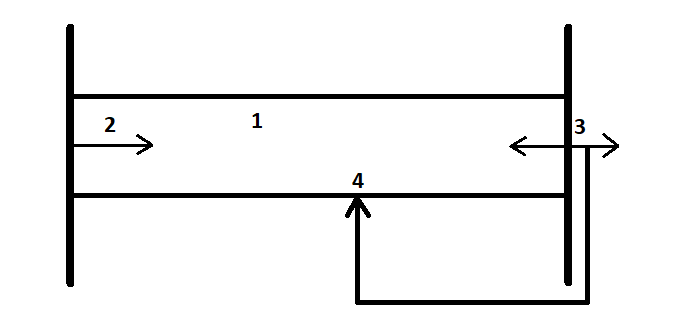
\includegraphics[scale=0.35]{Physical_model.png}  
\end{figure}

\vfill

\end{frame}

\begin{frame}
\frametitle{Модель изменения численности популяции животных}

$$
\dot{N} = \beta \, N'' + r(1 - N^2)N,
$$
$$
N'(0, t) \, = 0, \qquad N'(1, t) \, = \alpha\,N(x_0, t-\tilde{T}),
$$

\end{frame}

\begin{frame}
\frametitle{ Краевая задача с отклонением в краевом условии }

$$
\dot u = u'' + \gamma u - \delta u^3,	
$$
$$
u'(0, t) \, = 0, \qquad u'(1, t) \, = \alpha\,u(x_0, t) + (1 - \delta) \beta u^3(x_0, t),
$$
$$ t \geqslant 0, \quad x \in [0,1], \quad x_0 \in [0, 1), \quad  \delta \in \{0, 1\}, \quad \alpha,\,\beta,\,\gamma \in \mathbb{R}. $$

\vfill

\begin{itemize}

\item $ \delta = 1: $
\begin{equation}\label{problem_cube_in_eq}
	\dot u = u'' + \gamma u - u^3,	
\end{equation}
\begin{equation}\label{conditions_cube_in_eq}
	u'(0, t) \, = 0, \qquad u'(1, t) \, = \alpha\,u(x_0, t).
\end{equation}

\item $ \delta = 0: $
\begin{equation}\label{problem_cube_in_cond}
	\dot u = u'' + \gamma u,	
\end{equation}
\begin{equation}\label{conditions_cube_in_cond}
	u'(0, t) \, = 0, \qquad u'(1, t) \, = \alpha\,u(x_0, t) + \beta u^3(x_0, t).
\end{equation}

\end{itemize}

\end{frame}

\begin{frame}
\frametitle{ Линеаризованная краевая задача }

\begin{equation}\label{linear_problem}
	\dot u = u'' + \gamma u,	
\end{equation}
\begin{equation}\label{linear_conditions}
	u'(0, t) \, = 0, \qquad u'(1, t) \, = \alpha\,u(x_0, t).
\end{equation}

\vfill

$$ u(x, t) = e^{\lambda t} \, v(x). $$

\vfill
 
$$
v'' + (\gamma - \lambda)v = 0,
$$
$$
v'(0) \, = 0, \qquad v'(1) \, = \alpha\,v(x_0).
$$

\vfill

$$ v(x) = c \ch  \mu x, \qquad c \in \mathbb{R}, \quad \mu = \sqrt{-\gamma + \lambda}. $$

\end{frame}

\begin{frame}
\frametitle{ Потеря устойчивости нулевого решения }

\begin{itemize}

\item { $ \lambda = 0: \; \mu = \sqrt{-\gamma}, $ 
}

\begin{equation}\label{alpha_u}
	\alpha_u = \dfrac{ \sqrt{-\gamma} \, \sh \sqrt{-\gamma} }{ \ch \sqrt{-\gamma} x_0 }, 
\end{equation}

\item { $ \lambda = i \omega: \; \mu = \sqrt{-\gamma + i \omega}, $ 
}

\begin{equation}\label{alpha_c}
	\alpha_c = \frac{ \sqrt{-\gamma + i \omega} \, \sh \sqrt{-\gamma + i \omega} }{ \ch \sqrt{-\gamma + i \omega} x_0 }.
\end{equation}

\end{itemize}	

\begin{ruslemma}
Для линеаризованной в нуле системы дифференциальных уравнений \eqref{linear_problem}, \eqref{linear_conditions} нулевое состояние равновесия теряет свою устойчивость дивергентным способом для значений параметров $\alpha_u$ и $\gamma$, связанных между собой формулой \eqref{alpha_u} и колебательным, для значений параметров $\alpha_c$ и $\gamma$, связанных между собой уравнением \eqref{alpha_c}.
\end{ruslemma}

\end{frame}

\begin{frame}
\frametitle{Система ДУ с диффузионным взаимодействием}

$$ j = \overline{1, N} \qquad k \in [1,N]. $$

\begin{itemize}

\item $ \delta = 1: $
$$
\dot{u}_j =  N^2(u_{j+1} - 2u_j + u_{j-1}) + \gamma u_j - u_j^3,	
$$
$$ u_0 = u_1, \quad u_{N+1} = u_N + \frac{\alpha}{N}\:u_k. $$

\vfill

\item $ \delta = 0: $
$$
\dot{u}_j =  N^2(u_{j+1} - 2u_j + u_{j-1}) + \gamma u_j,	
$$
$$ u_0 = u_1, \quad u_{N+1} = u_N + \frac{\alpha}{N}\:u_k + \frac{\beta}{N}\:u_k^3. $$

\end{itemize}

\vfill

\begin{figure} 
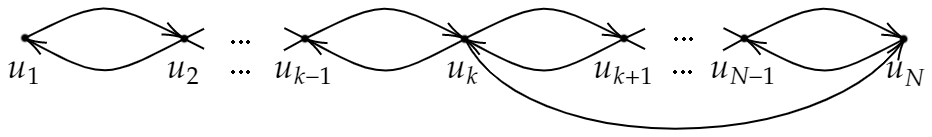
\includegraphics[scale=0.4]{chain.png}  
\end{figure}

\end{frame}

\begin{frame}
\frametitle{ Моделирование линейной краевой задачи }

$$ \dot{u}_j =  N^2(u_{j+1} - 2u_j + u_{j-1}) + \gamma u_j, \quad j = \overline{1, N}, $$
$$ u_0 = u_1, \qquad u_{N+1} = u_N + \frac{\alpha}{N}\:u_k, \quad k \in [1,N]. $$

\vfill
 
$$ u_j = e^{\lambda t} \ch \delta x_j, \qquad x_j = -\dfrac{1}{2N} + \dfrac{j}{N}. $$

\vfill

\begin{itemize}

\item { $ j \leqslant N-1: $ 
}
$$
\delta = 2N \arsh \dfrac{\sqrt{-\gamma+\lambda}}{2N}.
$$
\item { $ j = N: $ 
}
$$
\alpha = \dfrac{\sqrt{-\gamma+\lambda}\sh\delta}{\ch\delta x_k}.
$$

\end{itemize}

\end{frame}

\begin{frame}
\frametitle{ Потеря устойчивости нулевого решения }

\begin{itemize}

\item { $ \lambda = 0: $ 
}

$$ \alpha_u = \frac{ \sqrt{-\gamma} \, \sh \delta_u }{ \ch\delta_u x_k }, \qquad \delta_u = 2N \arsh \dfrac{\sqrt{-\gamma}}{2N}. $$

\medskip

\item { $ \lambda = \pm i \omega: \; $ 
}

$$ \alpha_c = \frac{ \sqrt{-\gamma + i \omega} \, \sh \delta_c }{ \ch\delta_c x_k }, \qquad \delta_c = 2N \arsh \dfrac{\sqrt{-\gamma + i \omega}}{2N}. $$

\end{itemize}

\bigskip

$$ N = 50. $$	

\end{frame}

\begin{frame}
\frametitle{ Построение зависимости $ \alpha_c(\gamma) $ }
 
\begin{itemize}

\item { $ \gamma = 0, \, x_0 = 0: $ 
$$
 \begin{cases}
   \tg \, y + \th \, y = 0, 
   \\
   \alpha_c = y(\sh y \cos y - \ch y \sin y).
 \end{cases}
$$
$$ y = \sqrt{ \frac{\omega}{2} }. $$
}

\item { $ \gamma = 0, \, x_0 \neq 0: $ 
$$
 \begin{cases}
   \dfrac{\sh y \cos y + \ch y \sin y}{\sh y \cos y - \ch y \sin y} - \tg y x_0 \th y x_0 = 0, 
   \vspace{0.1cm}
   \\ 
   \alpha_c = \dfrac{y \sh y \cos y - y \ch y \sin y}{\ch y x_0 \cos y x_0}.
 \end{cases}
$$
}

\item { $ \gamma \neq 0, \, x_0 \neq 0. $ 
}

\end{itemize}	

\end{frame}

\begin{frame}
\frametitle{ Численные результаты: $ \alpha_c(x_0) $ при $ \gamma = 0 $ }

\begin{figure} 
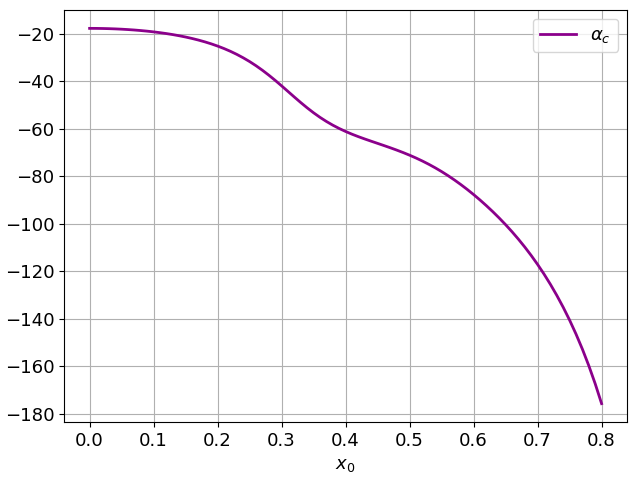
\includegraphics[scale=0.65]{origins.png}  
\end{figure}

\end{frame}

\begin{frame}
\frametitle{ Схематическая визуализация $ \alpha(\gamma) $ для $ 1 \leqslant k \leqslant 17 $ }

\begin{figure}[h]
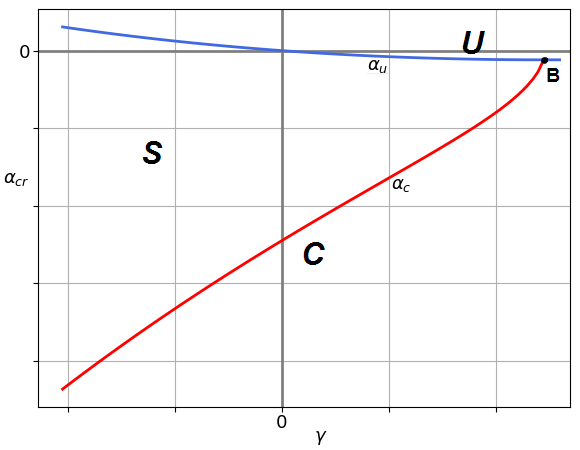
\includegraphics[scale=0.55]{k=1.png} 
\end{figure}

$$ k=1 \quad (x_0=0.01) $$

\end{frame}

\begin{frame}
\frametitle{ Схематическая визуализация $ \alpha(\gamma) $ для $ 18 \leqslant k \leqslant 23 $ }

\begin{figure}[h]
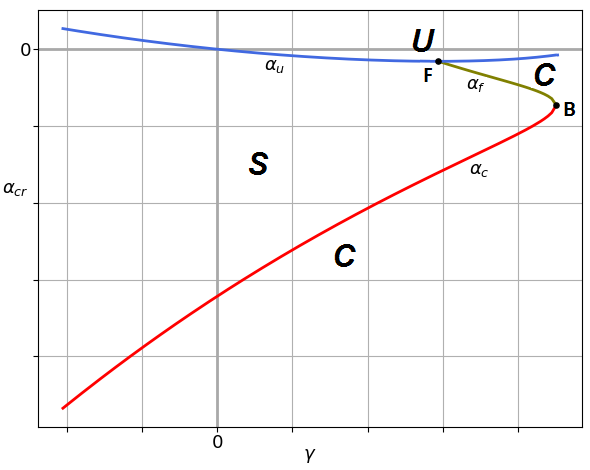
\includegraphics[scale=0.55]{k=22.png} 
\end{figure}

$$ k=22 \quad (x_0=0.43) $$

\end{frame}

\begin{frame}
\frametitle{ Схематическая визуализация $ \alpha(\gamma) $ для $ k=24 $ }

\begin{figure}[h]
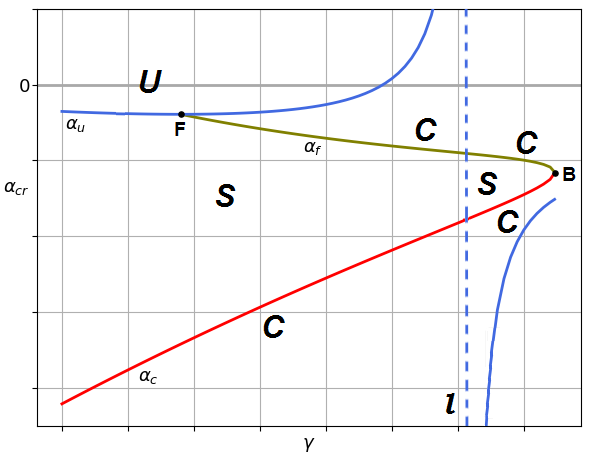
\includegraphics[scale=0.55]{k=24.png} 
\end{figure}

$$ k=24 \quad (x_0=0.47) $$

\end{frame}

\begin{frame}
\frametitle{ Схематическая визуализация $ \alpha(\gamma) $ для $ k=25 $ }

\begin{figure}[h]
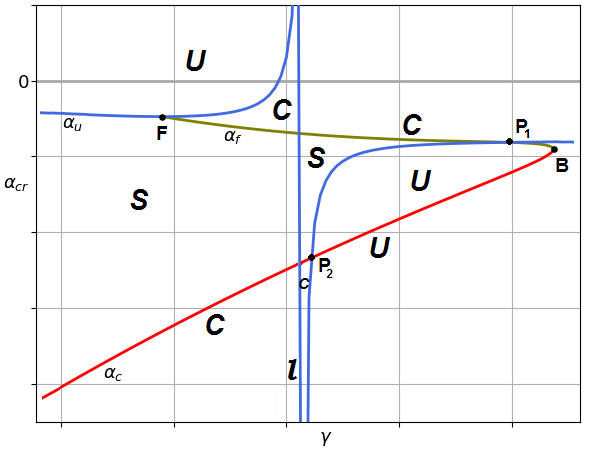
\includegraphics[scale=0.55]{k=25.png} 
\end{figure}

$$ k=25 \quad (x_0=0.49) $$

\end{frame}

\begin{frame}
\frametitle{ Схематическая визуализация $ \alpha(\gamma) $ для $ 26 \leqslant k \leqslant 32 $ }

\begin{figure}[h]
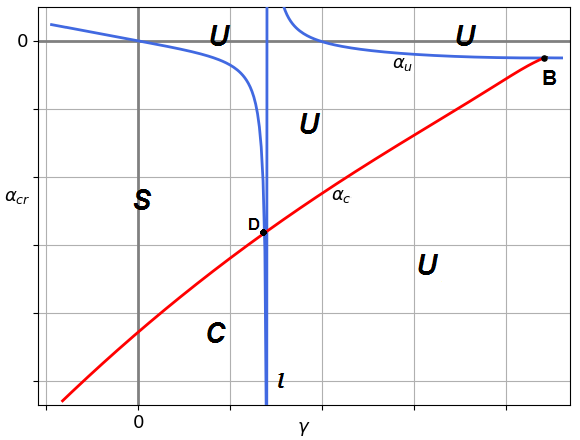
\includegraphics[scale=0.55]{k=26.png} 
\end{figure}

$$ k=26 \quad (x_0=0.51) $$

\end{frame}

\begin{frame}
\frametitle{ Схематическая визуализация $ \alpha(\gamma) $ для $ 33 \leqslant k \leqslant 38 $ }

\begin{figure}[h]
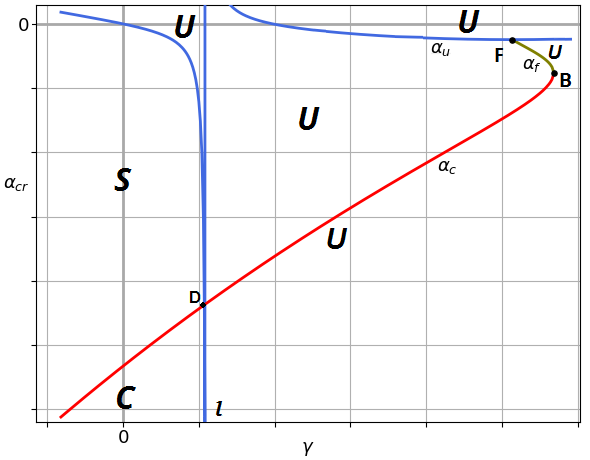
\includegraphics[scale=0.55]{k=34.png} 
\end{figure}

$$ k=34 \quad (x_0=0.67) $$

\end{frame}

\begin{frame}

\begin{equation}\label{Gamma_u}
    \Gamma_u =\left\{
                \begin{array}{ll}
                  \gamma_*, \quad 1 \leqslant k \leqslant 17,\\
                  \overline{\gamma}, \quad 18 \leqslant k \leqslant 25,\\
                  \hat{\gamma}, \quad 26 \leqslant k \leqslant 50.
                \end{array}
              \right.
\end{equation}

\vfill

\begin{equation}\label{Gamma_f}
    \Gamma_f =\left\{
                \begin{array}{ll}
                  \gamma_*, \quad 18 \leqslant k \leqslant 24,\\
                  \gamma_1, \quad k = 25.
                \end{array}
              \right.
\end{equation}

\vfill

\begin{equation}\label{Gamma_c}
    \Gamma_c =\left\{
                \begin{array}{ll}
                  \gamma_*, \quad 1 \leqslant k \leqslant 24,\\
                  \gamma_2, \quad k = 25,\\
                  \hat{\gamma}, \; \quad 26 \leqslant k \leqslant 50.
                \end{array}
              \right.
\end{equation}

\vfill

\begin{equation}\label{transcendent_equation_P}
\frac{\sqrt{-\gamma} \, \sh \delta_u}{\ch \delta_u x_{25}} - \frac{\sqrt{-\gamma + i \omega} \, \sh \delta_c}{\ch \delta_c x_{25}} = 0,
\end{equation}
\begin{equation}\label{transcendent_equation_cond}
    \gamma_* > \gamma_1 > \gamma_2 > l.
\end{equation}
$$ x_{25}=0.49. $$

\end{frame}

\begin{frame}

\begin{ruslemma}
Для всех значений $\gamma \leqslant \Gamma_u$, где $\Gamma_u$ определяется выражением \eqref{Gamma_u} и $\gamma_1 \geqslant \gamma \geqslant \gamma_2$, где $\gamma_1, \, \gamma_2$ являются корнями трансцендентного уравнения \eqref{transcendent_equation_P}, удовлетворяющими условию \eqref{transcendent_equation_cond}, критическая зависимость $\alpha_u(\gamma)$, рассчитываемая по формуле \eqref{alpha_u}, позволяет выделить область параметров $(\gamma, \, \alpha)$ с устойчивым нулевым решением систем \eqref{problem_cube_in_eq}, \eqref{conditions_cube_in_eq} и \eqref{problem_cube_in_cond}, \eqref{conditions_cube_in_cond} и области с двумя состояниями равновесия в малой окрестности неустойчивого нулевого решения.
\end{ruslemma}
\begin{ruslemma}
Для всех значений $\overline{\gamma} \leqslant \gamma \leqslant \Gamma_f$, где $\Gamma_f$ определяется выражением \eqref{Gamma_f}, и $\gamma \leqslant \Gamma_c$, где $\Gamma_c$ определяется выражением \eqref{Gamma_c}, критические зависимости $\alpha_f(\gamma)$ и $\alpha_c(\gamma)$, рассчитываемые по формуле \eqref{alpha_c}, позволяют выделить область параметров $(\gamma, \, \alpha)$ с устойчивым нулевым решением систем \eqref{problem_cube_in_eq}, \eqref{conditions_cube_in_eq} и \eqref{problem_cube_in_cond}, \eqref{conditions_cube_in_cond} и области, для которых наблюдается наличие цикла в малой окрестности неустойчивого нулевого решения.
\end{ruslemma}


\end{frame}

\begin{frame}
\frametitle{ Локальный анализ краевой задачи }

$$
u = \sqrt{\varepsilon}u_0 + \varepsilon u_1 + \varepsilon^{\frac{3}{2}} u_2 + O(\varepsilon^2).
$$

\vfill

$$ \varepsilon = | \alpha - \alpha_{cr} |, $$

$$ \varepsilon \ll 1, \quad s = \varepsilon t. $$

\end{frame}

\begin{frame}
\frametitle{ Краевая задача с лин. отклонением в краевом условии }

$$
\dot u = u'' + \gamma u - u^3,	
$$
$$
u'(0, t) \, = 0, \qquad u'(1, t) \, = \alpha\,u(x_0, t).
$$

\vfill

$$
\dot{u}_j =  N^2(u_{j+1} - 2u_j + u_{j-1}) + \gamma u_j - u_j^3, \quad j = \overline{1, N},
$$
$$ u_0 = u_1, \quad u_{N+1} = u_N + \frac{\alpha}{N}\:u_k. $$

\end{frame}

\begin{frame}
\frametitle{ Случай дивергентной потери устойчивости }

\begin{itemize}
\item { $ \lambda = 0: \quad \varepsilon=\alpha-\alpha_u, $
}
\end{itemize}

\vfill

$$
u_0 = u_0'' + \gamma u_0,
$$
$$
u_0'(0, t) \, = 0, \qquad u_0'(1, t) \, = \alpha_u u_0(x_0, t).
$$

$$ u_0 = \rho(s) \ch \sqrt{-\gamma} x. $$

\vfill

$$
\dot u_2 + \frac{\partial u_0}{\partial s} = u_2'' + \gamma u_2 - u_0^3,
$$
$$
u_2'(0, t) \, = 0, \qquad u_2'(1, t) \, = \alpha_u u_2(x_0, t) + u_0(x_0, t).
$$

$$ u_2 = e^{\lambda t}v_2(x). $$

\end{frame}

\begin{frame}
\frametitle{ Случай дивергентной потери устойчивости }

$$
\rho' = \phi_0 \rho + d_0 \rho^3.
$$

\vfill

$$ \phi_0 = \frac{ 2 \sqrt{-\gamma} \ch \sqrt{-\gamma} x_0 }{ \sqrt{-\gamma} \ch \sqrt{-\gamma} +\sh \sqrt{-\gamma} - \alpha_u x_0 \sh \sqrt{-\gamma} x_0 }, $$
$$ d_0 = -\frac{ 3\gamma \sh 3\sqrt{-\gamma} + \alpha_u \sqrt{-\gamma} \ch 3\sqrt{-\gamma} x_0 }{ 16( \sqrt{-\gamma} \ch \sqrt{-\gamma} +\sh \sqrt{-\gamma} - \alpha_u x_0 \sh \sqrt{-\gamma} x_0 ) } - \frac{3}{4}. $$

\end{frame}

\begin{frame}
\frametitle{ Случай дивергентной потери устойчивости }

\begin{itemize}
\item { $ \lambda = 0: \quad \varepsilon=\alpha-\alpha_u, $
}
\end{itemize}

$$
\dot u_{j,0} = N^2(u_{j+1,0} - 2u_{j,0} + u_{j-1,0}) + \gamma u_{j,0},
$$
$$
u_{0,0} = u_{1,0}, \quad u_{N+1,0} = u_{N,0} + \dfrac{\alpha}{N}u_{k,0}.
$$

\vfill

$$ u_{j,0} = \rho(s) \ch \delta_u x_j. $$

$$
\dot u_{j,2} + \frac{\partial u_{j,0}}{\partial s} = N^2(u_{j+1,2} - 2u_{j,2} + u_{j-1,2}) + \gamma u_{j,2} - u_{j,0}^3,
$$
$$
u_{0,2} = u_{1,2}, \quad u_{N+1,2} = u_{N,2} + \dfrac{\alpha}{N}u_{k,0}.
$$

\vfill

$$ u_{j,2} = \ch \delta_u x_j. $$

\end{frame}

\begin{frame}
\frametitle{ Случай дивергентной потери устойчивости }

$$ \rho' = \phi_0 \rho + d_0 \rho^3. $$

\vfill

$$ \phi_0 = \frac{ 2 \delta_u \ch \delta_u x_k }{ \delta_u \ch \delta_u +\sh \delta_u - \alpha_u x_k \sh \delta_u x_k }, $$
$$ d_0 = -\frac{ 3\delta_u^2 \sh 3\delta_u + \alpha_u \delta_u \ch 3\delta_u x_k }{ 16( \delta_u \ch \delta_u +\sh \delta_u - \alpha_u x_k \sh \delta_u x_k ) } - \frac{3}{4}. $$

\vfill

$$ \alpha_u = \frac{ \sqrt{-\gamma} \, \sh \delta_u }{ \ch\delta_u x_k }, \qquad \delta_u = 2N \arsh \dfrac{\sqrt{-\gamma}}{2N}, \quad x_j = -\dfrac{1}{2N} + \dfrac{j}{N}. $$

\end{frame}

\begin{frame}
\frametitle{ Численные результаты: $ \phi_0(\gamma) $ и $ d_0(\gamma) $ }

\begin{center}
\begin{tabular}{cc}
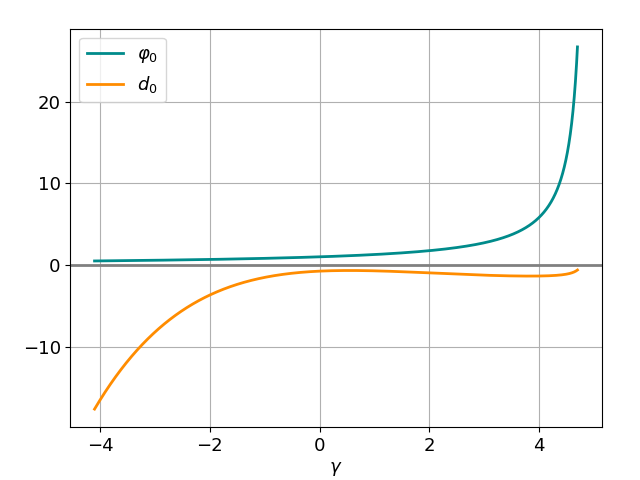
\includegraphics[scale=0.32]{divergent_phi0d0_033.png} &
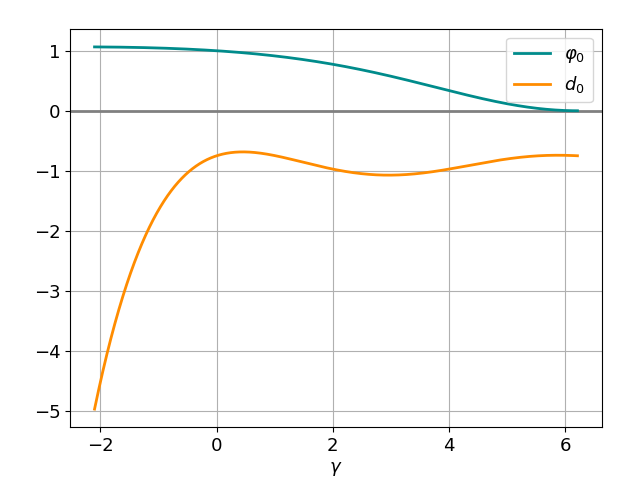
\includegraphics[scale=0.32]{divergent_phi0d0_063.png} \\
\small{$k=17\;(x_0=0.33)$ } & \small{$k=32\;(x_0=0.63)$ } \\
\end{tabular}
\end{center}

\vfill

$$ \gamma<\Gamma_0, $$

\vfill

\begin{equation}\label{Gamma_0}
    \Gamma_0 =\left\{
                \begin{array}{ll}
                  \tilde{\gamma}, \qquad 1 \leqslant k \leqslant 25,\\
                  \Gamma_u, \quad 25 \leqslant k \leqslant 50,
                \end{array}
              \right.
\end{equation}
$$ -\frac{ 3\delta_u^2 \sh 3\delta_u + \alpha_u \delta_u \ch 3\delta_u x_k }{ 16( \delta_u \ch \delta_u +\sh \delta_u - \alpha_u x_k \sh \delta_u x_k ) } - \frac{3}{4} = 0.$$

\end{frame}

\begin{frame}
\frametitle{ Численные результаты: $ d_0(\gamma) $ }

\begin{center}
\begin{tabular}{cc}
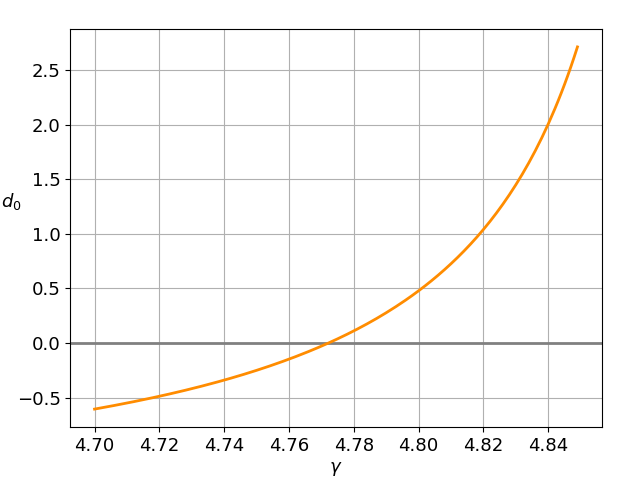
\includegraphics[scale=0.32]{divergent_d0_033.png} &
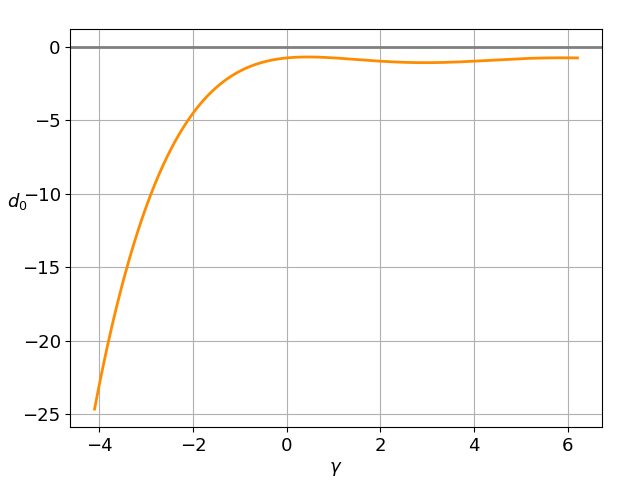
\includegraphics[scale=0.32]{divergent_d0_063.png} \\
\small{$k=17\;(x_0=0.33)$ } & \small{$k=32\;(x_0=0.63)$ } \\
\end{tabular}
\end{center}

\vfill

$$ \gamma<\gamma_*, $$

\vfill

\begin{equation}\label{asymptotic_div}
    u_j = \pm \sqrt{-\varepsilon \, \dfrac{\phi_0}{d_0}} \ch \delta_u x_j + O(\varepsilon).
\end{equation}

\end{frame}

\begin{frame}

\begin{rustheorem}
Пусть $ \varepsilon = \alpha - \alpha_u$, для $ \gamma \leqslant \Gamma_0 $, где $ \Gamma_0 $ вычисляется по формуле \eqref{Gamma_0}. Тогда для любого $ \gamma \leqslant \Gamma_0 $ существует $ \varepsilon_0 $ такое, что для $ \varepsilon \in (0, \varepsilon_0] $ система дифференциальных уравнений \eqref{problem_cube_in_eq}, \eqref{conditions_cube_in_eq} имеет в окрестности неустойчивого нулевого решения два пространственно неоднородных устойчивых режима, асимптотика которых определяется формулой \eqref{asymptotic_div}.
\end{rustheorem}
\begin{rustheorem}
Пусть $ \varepsilon = \alpha - \alpha_u$, для $ \Gamma_0 \leqslant \gamma \leqslant \Gamma_u $, где $ \Gamma_0$ и $\Gamma_u $ вычисляются по формулам \eqref{Gamma_0} и \eqref{Gamma_u} соответственно. Тогда для любого $ \Gamma_0 < \gamma \leqslant \Gamma_u $ существует $ \varepsilon_0 $ такое, что для $ \varepsilon \in (0, \varepsilon_0] $ система дифференциальных уравнений \eqref{problem_cube_in_eq}, \eqref{conditions_cube_in_eq} имеет неустойчивое нулевое решение, которое грубо теряет свою устойчивость в результате приближения к нему двух пространственно неоднородных устойчивых состояний равновесия, асимптотика которых определяется формулой \eqref{asymptotic_div}.
\end{rustheorem}

\end{frame}

\begin{frame}
\frametitle{ Численные результаты: $ \phi_0(\gamma) $ и $ d_0(\gamma) $ для $ k=25 $ }

$$ \varepsilon = \alpha_u - \alpha: \qquad \phi_0 \longmapsto -\phi_0. $$

\vfill

\begin{figure}[h]
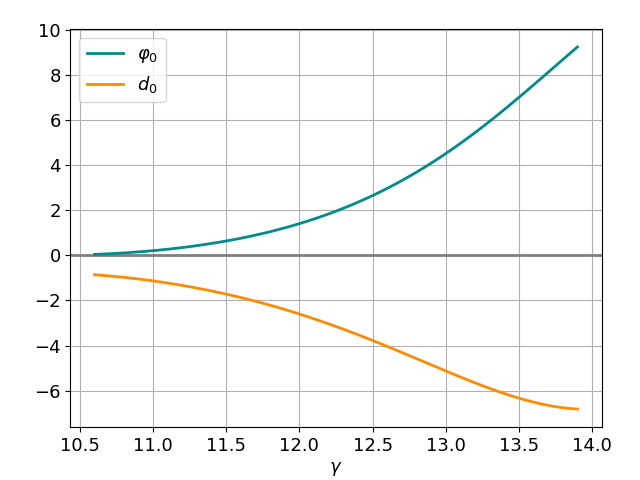
\includegraphics[scale=0.4]{divergent_phi0d0_049_P.png} 
\end{figure}
$$ k=25 \; (x_0=0.49) $$

\vfill

$$ \gamma_1 > \gamma > \gamma_2. $$

\end{frame}

\begin{frame}

\begin{rustheorem}
Пусть $ \varepsilon = \alpha_u - \alpha $ для $\gamma_1 \geqslant \gamma \geqslant \gamma_2$, где $\gamma_1$ и $\gamma_2$ являются корнями трансцендентного уравнения \eqref{transcendent_equation_P}, удовлетворяющими условию \eqref{transcendent_equation_cond}. Тогда для любого $\gamma_1 > \gamma > \gamma_2$ существует $ \varepsilon_0 $ такое, что для $ \varepsilon \in (0, \varepsilon_0] $ система дифференциальных уравнений \eqref{problem_cube_in_eq}, \eqref{conditions_cube_in_eq} имеет в окрестности неустойчивого нулевого решения два пространственно неоднородных устойчивых режима, асимптотика которых определяется формулой \eqref{asymptotic_div}.
\end{rustheorem}

\end{frame}

\begin{frame}
\frametitle{ Случай колебательной потери устойчивости }

\begin{itemize}
\item { $ \lambda = \pm i \omega: \quad \varepsilon=\alpha_c-\alpha, $
}
\end{itemize}

\vfill

$$
u_0 = u_0'' + \gamma u_0,
$$
$$
u_0'(0, t) \, = 0, \qquad u_0'(1, t) \, = \alpha_c u_0(x_0, t).
$$

$$ u_0 = z(s) e^{i \omega t} \ch \mu x + \overline{z(s)} e^{-i \omega t} \overline{\ch \mu x}. $$

\vfill

$$
\dot u_2 + \frac{\partial u_0}{\partial s} = u_2'' + \gamma u_2 - u_0^3,
$$
$$
u_2'(0, t) \, = 0, \qquad u_2'(1, t) \, = \alpha_c u_2(x_0, t) + u_0(x_0, t).
$$

$$ u_2(x) = \ch \sqrt{-\gamma + i \omega} \, x. $$

\end{frame}


\begin{frame}
\frametitle{ Случай колебательной потери устойчивости }

$$
z' = \phi_0 z + d_0 z |z|^2.
$$

\bigskip

$$ \phi_0 = -\operatorname{Re} \left( \frac{ 2 \mu \ch \mu x_0 }{ \mu \ch \mu +\sh \mu - \alpha_c x_0 \sh \mu x_0 } \right), $$

$$ d_0 = \operatorname{Re} \left( \frac{ 3 \mu ( G(\mu + 2\,\mbox{Re}\mu) + G(\mu + 2i\,\mbox{Im}\mu) + 2G(\overline{\mu}) ) }{ 2 ( \mu \ch \mu +\sh \mu - \alpha_c x_0 \sh \mu x_0 ) } \right). $$

$$ \mu = \sqrt{-\gamma + i \omega}, $$

$$ G(y) = \frac{ \alpha_c - y\,\sh y }{ y^2 + \gamma - i\omega }. $$

\end{frame}

\begin{frame}
\frametitle{ Случай колебательной потери устойчивости }

\begin{itemize}
\item { $ \lambda = \pm i \omega: \quad \varepsilon=\alpha_c-\alpha, $
}
\end{itemize}

$$
\dot u_{j,0} = N^2(u_{j+1,0} - 2u_{j,0} + u_{j-1,0}) + \gamma u_{j,0},
$$
$$
u_{0,0} = u_{1,0}, \quad u_{N+1,0} = u_{N,0} + \dfrac{\alpha}{N}u_{k,0}.
$$

\vfill

$$ u_{j,0} = z(s) e^{i \omega t} \ch \delta_c x_j + \overline{z(s)} e^{-i \omega t} \overline{\ch \delta_c x_j}. $$

$$
\dot u_{j,2} + \frac{\partial u_{j,0}}{\partial s} = N^2(u_{j+1,2} - 2u_{j,2} + u_{j-1,2}) + \gamma u_{j,2} - u_{j,0}^3,
$$
$$
u_{0,2} = u_{1,2}, \quad u_{N+1,2} = u_{N,2} + \dfrac{\alpha}{N}u_{k,0}.
$$

\vfill

$$ u_{j,2} = e^{i \omega t} \ch \delta_c x_j. $$

\end{frame}

\begin{frame}
\frametitle{ Случай колебательной потери устойчивости }

\begin{equation}
	z' = \phi_0 z + d_0 z |z|^2,
\end{equation}

\vfill

$$ \phi_0 = \mbox{Re} \left(\dfrac{2 \delta_c \ch \delta_c x_k}{\delta_c\ch \delta_c + \sh \delta_c - \alpha_c x_k \sh \delta_c x_k} \right), $$
$$ d_0 = \mbox{Re} \left( \dfrac{3 \delta_c (G(\delta_c + 2 \mbox{Re}\,\delta) + G(\delta_c + 2 \mbox{Im}\,\delta_c) + 2G(\overline{\delta_c}) )}{2(\delta_c\ch \delta_c + \sh \delta_c - \alpha_c x_k \sh \delta_c x_k)} \right). $$

\vfill

$$ \alpha_c = \frac{ \sqrt{-\gamma + i \omega} \, \sh \delta_c }{ \ch\delta_c x_k }, \quad  \delta_c = 2N \arsh \dfrac{\sqrt{-\gamma + i \omega}}{2N}, \quad x_j = -\dfrac{1}{2N} + \dfrac{j}{N}. $$

\end{frame}

\begin{frame}
\frametitle{ Численные результаты: $ \phi_0(\gamma) $ и $ d_0(\gamma) $ }

\begin{center}
\begin{tabular}{cc}
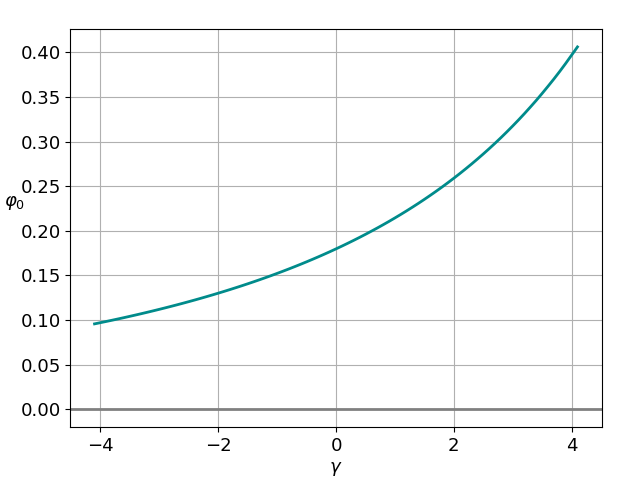
\includegraphics[scale=0.32]{oscillating_phi0_000.png} &
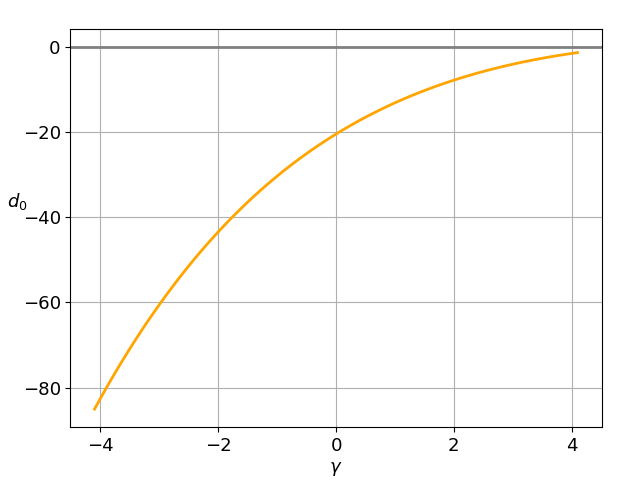
\includegraphics[scale=0.32]{oscillating_d0_000.png} \\
\end{tabular}
\end{center}

\vfill

$$k=1 \; (x_0 =0.01) $$

$$ \gamma < \Gamma_c $$

\end{frame}

\begin{frame}

$$ z=\varrho e^{i \nu}. $$

\vfill

$$
\varrho' = \phi_0 \varrho + d_0 \varrho^3,
$$
$$
\nu' = \psi_0 + c_0 \nu^2.
$$

\vfill

$$ \lim_{s \rightarrow +\infty} \varrho = \sqrt{-\dfrac{\phi_0}{d_0}}. $$

\vfill

$$
\nu(s) = \sigma s + \gamma, \qquad \sigma = \frac{\psi_0 d_0 - c_0 \phi_0}{d_0}.
$$

\vfill

\begin{equation}\label{asymptotic_osc}
    u_j = \sqrt{-\varepsilon\, \dfrac{\phi_0}{d_0}} \left( e^{i A t} \, \ch \delta_c x_j + e^{-i A t} \, \overline{\ch \delta_c x_j}  \right) + O(\varepsilon).
\end{equation}
$$ A = \omega + \varepsilon \sigma $$

\end{frame}

\begin{frame}

\begin{rustheorem}
Пусть $ \varepsilon = \alpha_c - \alpha $ для $ \gamma \leqslant \Gamma_c $, где $ \Gamma_c $ вычисляется с помощью \eqref{Gamma_c}. Тогда для любого $ \gamma < \Gamma_c $ существует $ \varepsilon_0 $ такое, что для $ \varepsilon \in (0, \varepsilon_0] $ система дифференциальных уравнений \eqref{problem_cube_in_eq}, \eqref{conditions_cube_in_eq} имеет в окрестности нуля орбитально инвариантный устойчивый цикл с асимптотикой \eqref{asymptotic_osc}.
\end{rustheorem}

\end{frame}

\begin{frame}
\frametitle{ Численные результаты: $ \phi_0(\gamma) $ и $ d_0(\gamma) $ }

$$ \varepsilon = \alpha_f - \alpha: \qquad a_c \longmapsto a_f, \; \phi_0 \longmapsto -\phi_0. $$

\vfill

\begin{center}
\begin{tabular}{cc}
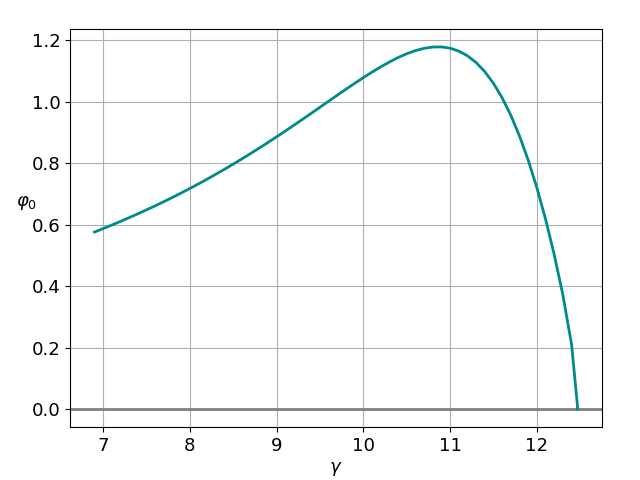
\includegraphics[scale=0.32]{oscillating_phi0_after_tangent_047.png} &
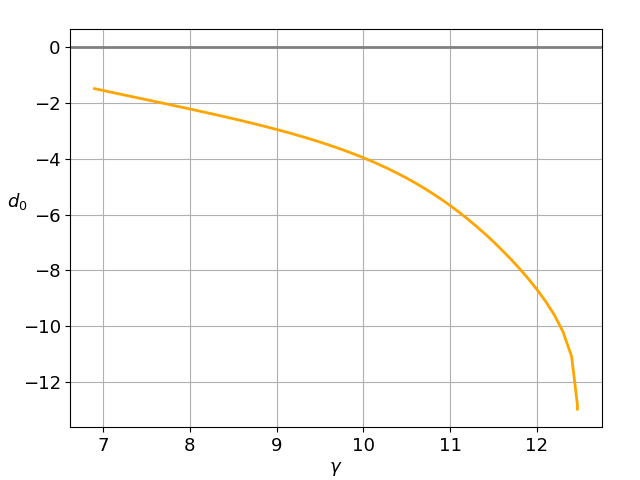
\includegraphics[scale=0.32]{oscillating_d0_after_tangent_047.png} \\
\end{tabular}
\end{center}
$$ k=24 \; (x_0=0.47) $$

\vfill

$$ \overline{\gamma} < \gamma < \Gamma_f. $$

\end{frame}

\begin{frame}

\begin{rustheorem}
Пусть $ \varepsilon = \alpha - \alpha_f $ для $ \overline{\gamma} \leqslant \gamma \leqslant \Gamma_f $, где $ \Gamma_f $ вычисляется с помощью \eqref{Gamma_f}. Тогда для любого $ \overline{\gamma} < \gamma < \Gamma_f $ существует $ \varepsilon_0 $ такое, что для $ \varepsilon \in (0, \varepsilon_0] $ система дифференциальных уравнений \eqref{problem_cube_in_eq}, \eqref{conditions_cube_in_eq} имеет в окрестности нуля орбитально инвариантный устойчивый цикл с асимптотикой \eqref{asymptotic_osc}.
\end{rustheorem}

\end{frame}

\begin{frame}
\frametitle{ Краевая задача с куб. отклонением в краевом условии }

$$
\dot u = u'' + \gamma u,	
$$
$$
u'(0, t) \, = 0, \qquad u'(1, t) \, = \alpha\,u(x_0, t) + \beta u^3(x_0, t).
$$

\vfill

$$
\dot{u}_j =  N^2(u_{j+1} - 2u_j + u_{j-1}) + \gamma u_j, \quad j = \overline{1, N},
$$
$$ u_0 = u_1, \quad u_{N+1} = u_N + \frac{\alpha}{N}\:u_k + \frac{\beta}{N}\:u_k^3. $$

\end{frame}

\begin{frame}
\frametitle{ Случай дивергентной потери устойчивости }

\begin{itemize}
\item { $ \lambda = 0: \quad \varepsilon=\alpha-\alpha_u, $
}
\end{itemize}

\vfill

$$
u_0 = u_0'' + \gamma u_0,
$$
$$
u_0'(0, t) \, = 0, \qquad u_0'(1, t) \, = \alpha_u u_0(x_0, t).
$$

$$ u_0 = \rho(s) \ch \sqrt{-\gamma} x. $$

\vfill

$$
\dot u_2 + \frac{\partial u_0}{\partial s} = u_2'' + \gamma u_2,
$$
$$
u_2'(0, t) \, = 0, \qquad u_2'(1, t) \, = \alpha_u u_2(x_0, t) + u_0(x_0, t) + \beta u_0^3(x_0, t).
$$

\vfill

$$ u_2 = e^{\lambda t}v_2(x). $$

\end{frame}

\begin{frame}
\frametitle{ Случай дивергентной потери устойчивости }

$$
\rho' = \phi_0 \rho + d_0 \rho^3.
$$

\vfill

$$ \phi_0 = Q \ch \sqrt{-\gamma} x_0, \qquad d_0 = \beta Q \ch^3 \sqrt{-\gamma} x_0. $$

$$ Q = \frac{2\sqrt{-\gamma}}{\sqrt{-\gamma}\ch\sqrt{-\gamma} + \sh\sqrt{-\gamma} - \alpha_u x_0 \sqrt{-\gamma} x_0}. $$

\end{frame}

\begin{frame}
\frametitle{ Случай дивергентной потери устойчивости }

\begin{itemize}
\item { $ \lambda = 0: \quad \varepsilon=\alpha-\alpha_u, $
}
\end{itemize}

$$
\dot u_{j,0} = N^2(u_{j+1,0} - 2u_{j,0} + u_{j-1,0}) + \gamma u_{j,0},
$$
$$
u_{0,0} = u_{1,0}, \quad u_{N+1,0} = u_{N,0} + \dfrac{\alpha}{N}u_{k,0}.
$$

\vfill

$$ u_{j,0} = \rho(s) \ch \delta_u x_j, $$

$$
\dot u_{j,2} + \frac{\partial u_{j,0}}{\partial s} = N^2(u_{j+1,2} - 2u_{j,2} + u_{j-1,2}) + \gamma u_{j,2},
$$
$$
u_{0,2} = u_{1,2}, \quad u_{N+1,2} = u_{N,2} + \dfrac{\alpha}{N}u_{k,0} + \dfrac{\beta}{N}u_{k,0}.
$$

\vfill

$$ u_{j,2} = \ch \delta_u x_j. $$

\end{frame}

\begin{frame}
\frametitle{ Случай дивергентной потери устойчивости }

$$ \rho' = \phi_0 \rho + d_0 \rho^3. $$

\vfill

$$ \phi_0 = Q \ch \delta_u x_k, \qquad d_0 = \beta Q \ch^3 \delta_u x_k. $$

$$ Q = \frac{2 \delta_u}{\delta_u\ch \delta_u + \sh \delta_u - \alpha_u x_k \sh \delta_u x_k}. $$

\vfill

$$ \alpha_u = \frac{ \sqrt{-\gamma} \, \sh \delta_u }{ \ch\delta_u x_k }, \qquad \delta_u = 2N \arsh \dfrac{\sqrt{-\gamma}}{2N}, \quad x_j = -\dfrac{1}{2N} + \dfrac{j}{N}. $$

\end{frame}

\begin{frame}
\frametitle{ Численные результаты: $ \phi_0(\gamma) $ и $ d_0(\gamma) $ }

\begin{figure} 
\begin{minipage}[h]{0.49\linewidth}
\begin{center}
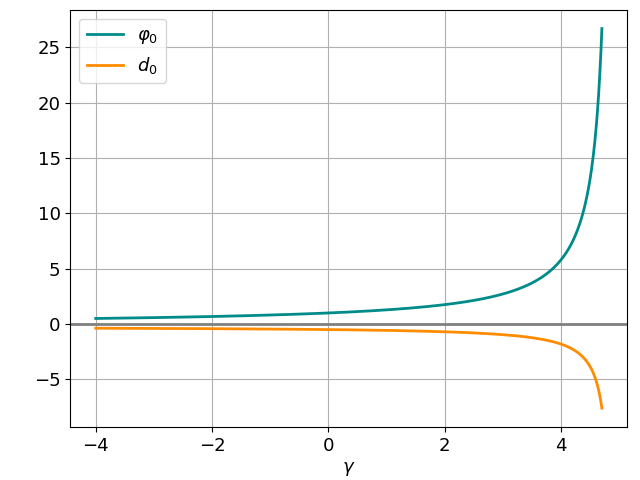
\includegraphics[scale=0.34]{divergent_phi0d0_x0=0,33,beta=-0,5.png} \\ {\scriptsize a) $ \beta = -0.5 $}
\end{center}
\end{minipage} 
\hfill
\begin{minipage}[h]{0.49\linewidth}
\begin{center}
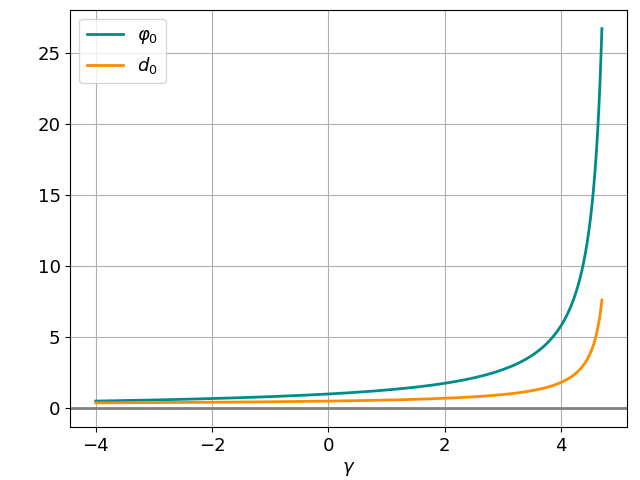
\includegraphics[scale=0.34]{divergent_phi0d0_x0=0,33,beta=0,5.png}  \\ {\scriptsize b) $ \beta = 0.5 $}
\end{center}
\end{minipage} 
\end{figure}

$$ k=17 \; (x_0 = 0.33) $$

$$ \gamma < \Gamma_u $$

\end{frame}

\begin{frame}

\begin{rustheorem}
Пусть $\beta<0$, а $\varepsilon = \alpha - \alpha_u$, для $\gamma \leqslant \Gamma_u$, где $\Gamma_u$ вычисляется по формуле \eqref{Gamma_u}. Тогда для любого $\gamma < \Gamma_u$ существует $\varepsilon_0$ такое, что для $\varepsilon \in (0, \varepsilon_0]$ система \eqref{problem_cube_in_cond}, \eqref{conditions_cube_in_cond} имеет в окрестности неустойчивого нулевого решения два пространственно неоднородных устойчивых режима, асимптотика которых определяется формулой \eqref{asymptotic_div}.
\end{rustheorem}
\begin{rustheorem}
Пусть $\beta>0$, а $\varepsilon = \alpha - \alpha_u$, для $\gamma \leqslant \Gamma_u$, где $\Gamma_u$ вычисляется по формуле \eqref{Gamma_u}. Тогда для любого $\gamma < \Gamma_u$ существует $\varepsilon_0$ такое, что для $\varepsilon \in (0, \varepsilon_0]$ система \eqref{problem_cube_in_cond}, \eqref{conditions_cube_in_cond} имеет неустойчивое нулевое решение, которое грубо теряет свою устойчивость в результате приближения к нему двух пространственно неоднородных устойчивых состояний равновесия, асимптотика которых определяется формулой \eqref{asymptotic_div}.
\end{rustheorem}

\end{frame}

\begin{frame}
\frametitle{ Численные результаты: $ \phi_0(\gamma) $ и $ d_0(\gamma) $ }

$$ \varepsilon = \alpha_u - \alpha: \qquad \phi_0 \longmapsto -\phi_0. $$

\vfill

\begin{figure}[h]
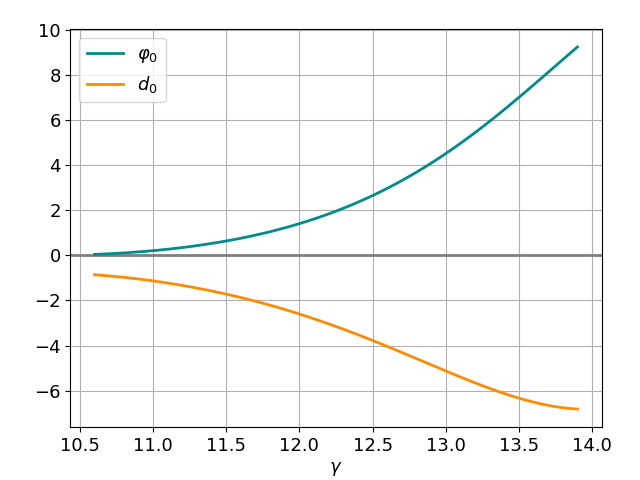
\includegraphics[scale=0.4]{divergent_phi0d0_049_P.png} 
\end{figure}
$$ k=25 \; (x_0=0.49) $$

\vfill

$$ \gamma_1 > \gamma > \gamma_2. $$

\end{frame}

\begin{frame}

\begin{rustheorem}
Пусть $\beta<0$, а $ \varepsilon = \alpha_u - \alpha $ для $\gamma_1 \geqslant \gamma \geqslant \gamma_2$, где $\gamma_1$ и $\gamma_2$ являются корнями трансцендентного уравнения \eqref{transcendent_equation_P}, удовлетворяющими условию \eqref{transcendent_equation_cond}. Тогда для любого $\gamma_1 > \gamma > \gamma_2$ существует $ \varepsilon_0 $ такое, что для $ \varepsilon \in (0, \varepsilon_0] $ система \eqref{problem_cube_in_cond}, \eqref{conditions_cube_in_cond} имеет в окрестности нуля два пространственно неоднородных неустойчивых режима, асимптотика которых определяется формулой \eqref{asymptotic_div}.
\end{rustheorem}
\begin{rustheorem}
Пусть $\beta>0$, а $ \varepsilon = \alpha_u - \alpha $ для $\gamma_1 \geqslant \gamma \geqslant \gamma_2$, где $\gamma_1$ и $\gamma_2$ являются корнями трансцендентного уравнения \eqref{transcendent_equation_P}, удовлетворяющими условию \eqref{transcendent_equation_cond}. Тогда для любого $\gamma_1 > \gamma > \gamma_2$ существует $\varepsilon_0$ такое, что для $\varepsilon \in (0, \varepsilon_0]$ система \eqref{problem_cube_in_cond}, \eqref{conditions_cube_in_cond} имеет неустойчивое нулевое решение, которое грубо теряет свою устойчивость в результате приближения к нему двух пространственно неоднородных устойчивых состояний равновесия, асимптотика которых определяется формулой \eqref{asymptotic_div}.
\end{rustheorem}

\end{frame}

\begin{frame}
\frametitle{ Случай колебательной потери устойчивости }

\begin{itemize}
\item { $ \lambda = \pm i \omega: \quad \varepsilon=\alpha_c-\alpha, $
}
\end{itemize}

\vfill

$$
u_0 = u_0'' + \gamma u_0,
$$
$$
u_0'(0, t) \, = 0, \qquad u_0'(1, t) \, = \alpha_c u_0(x_0, t).
$$

$$ u_0 = z(s) e^{i \omega t} \ch \mu x + \overline{z(s)} e^{-i \omega t} \overline{\ch \mu x}. $$

\vfill

$$
\dot u_2 + \frac{\partial u_0}{\partial s} = u_2'' + \gamma u_2,
$$
$$
u_2'(0, t) \, = 0, \qquad u_2'(1, t) \, = \alpha_c u_2(x_0, t) - u_0(x_0, t) + \beta u_0^3(x_0, t).
$$

\vfill

$$ u_2 = e^{i \omega t} v_2(x). $$

\end{frame}

\begin{frame}
\frametitle{ Случай колебательной потери устойчивости }

$$
z' = \phi_0 z + d_0 z |z|^2.
$$

\vfill

$$ \phi_0 = \mbox{Re} \left(\dfrac{2 \mu \ch \mu x_0}{\mu \ch \mu + \sh \mu - \alpha_f x_0 \sh \mu x_0} \right), $$

$$ d_0 = \mbox{Re} \left( \dfrac{3 \beta \mu (\ch (\mu + 2\,\mbox{Re}\,\mu) x_0 + \ch (\mu + 2 \,\mbox{Im}\,\mu) x_0 + 2 \ch \overline{\mu} x_0)}{2(\mu \ch \mu + \sh \mu - \alpha_f x_0 \sh \mu x_0)} \right). $$

\vfill

$$ \mu = \sqrt{-\gamma + i \omega}. $$

\end{frame}

\begin{frame}
\frametitle{ Случай колебательной потери устойчивости }

\begin{itemize}
\item { $ \lambda = \pm i \omega: \quad \varepsilon=\alpha_c-\alpha, $
}
\end{itemize}

$$
\dot u_{j,0} = N^2(u_{j+1,0} - 2u_{j,0} + u_{j-1,0}) + \gamma u_{j,0},
$$
$$
u_{0,0} = u_{1,0}, \quad u_{N+1,0} = u_{N,0} + \dfrac{\alpha}{N}u_{k,0}.
$$

\vfill

$$ u_{j,0} = z(s) e^{i \omega t} \ch \delta_c x_j + \overline{z(s)} e^{-i \omega t} \overline{\ch \delta_c x_j}. $$

$$
\dot u_{j,2} + \frac{\partial u_{j,0}}{\partial s} = N^2(u_{j+1,2} - 2u_{j,2} + u_{j-1,2}) + \gamma u_{j,2},
$$
$$
u_{0,2} = u_{1,2}, \quad u_{N+1,2} = u_{N,2} + \dfrac{\alpha}{N}u_{k,0} + \dfrac{\beta}{N}u_{k,0}.
$$

\vfill

$$ u_{j,2} = e^{i \omega t} \ch \delta_c x_j. $$

\end{frame}

\begin{frame}
\frametitle{ Случай колебательной потери устойчивости }

\begin{equation}
	z' = \phi_0 z + d_0 z |z|^2,
\end{equation}

\vfill

$$ \phi_0 = -\mbox{Re} \left(\dfrac{2 \delta_c \ch \delta_c x_k}{\delta_c\ch \delta_c + \sh \delta_c - \alpha_c x_k \sh \delta_c x_k} \right), $$
$$ d_0 = \mbox{Re} \left( \dfrac{3 \beta \delta_c (\ch (\delta_c + 2\mbox{Re}\:\delta_c) x_k + \ch (\delta_c + 2i\:\mbox{Im}\:\delta_c) x_k + 2 \ch \overline{\delta_c} x_k)}{2(\delta_c\ch \delta_c + \sh \delta_c - \alpha_c x_k \sh \delta_c x_k)} \right). $$

\vfill

$$ \alpha_c = \frac{ \sqrt{-\gamma + i \omega} \, \sh \delta_c }{ \ch\delta_c x_k }, \quad  \delta_c = 2N \arsh \dfrac{\sqrt{-\gamma + i \omega}}{2N}, \quad x_j = -\dfrac{1}{2N} + \dfrac{j}{N}. $$

\end{frame}

\begin{frame}
\frametitle{ Численные результаты: $ \phi_0(\gamma) $ и $ d_0(\gamma) $ }

\begin{figure} 
\begin{minipage}[h]{0.49\linewidth}
\begin{center}
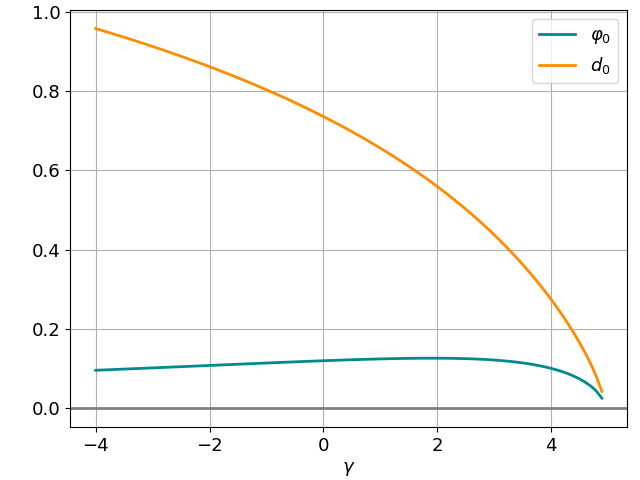
\includegraphics[scale=0.33]{oscillating_phi0d0_x0=0,33,beta=-1,0.png} \\ {\scriptsize a) $ \beta = -1.0 $}
\end{center}
\end{minipage} 
\hfill
\begin{minipage}[h]{0.49\linewidth}
\begin{center}
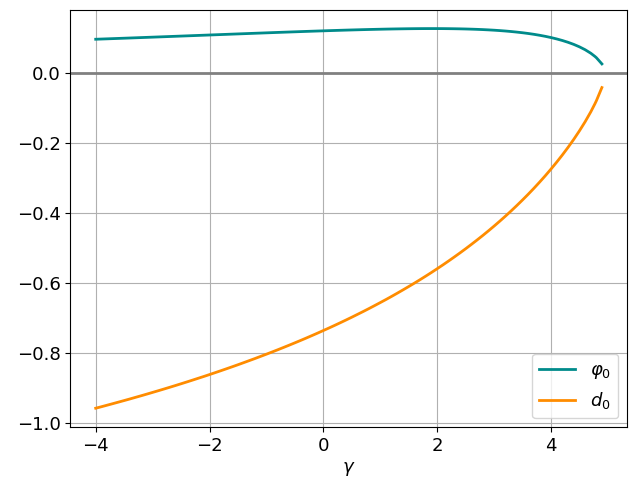
\includegraphics[scale=0.33]{oscillating_phi0d0_x0=0,33,beta=1,0.png}  \\ {\scriptsize b) $ \beta = 1.0 $}
\end{center}
\end{minipage} 
\end{figure}

$$ x_0 = 0.33 $$

\end{frame}

\begin{frame}

\begin{rustheorem}
Пусть $\beta<0$, а $ \varepsilon = \alpha_c - \alpha $ для $\gamma \geqslant \Gamma_c$, где $\Gamma_c$ вычисляется по формуле \eqref{Gamma_c}. Тогда для любого $\gamma < \Gamma_c$ существует $ \varepsilon_0 $ такое, что для $ \varepsilon \in (0, \varepsilon_0] $ система \eqref{problem_cube_in_cond}, \eqref{conditions_cube_in_cond} имеет в окрестности нуля орбитально инвариантный устойчивый цикл с асимптотикой \eqref{asymptotic_osc}.
\end{rustheorem}
\begin{rustheorem}
Пусть $\beta>0$, а $ \varepsilon = \alpha_c - \alpha $ для $\gamma \geqslant \Gamma_c$, где $\Gamma_c$ вычисляется по формуле \eqref{Gamma_c}. Тогда для любого $\gamma < \Gamma_c$ существует $ \varepsilon_0 $ такое, что для $ \varepsilon \in (0, \varepsilon_0] $ система \eqref{problem_cube_in_cond}, \eqref{conditions_cube_in_cond} имеет в окрестности нуля орбитально инвариантный неустойчивый цикл с асимптотикой \eqref{asymptotic_osc}.
\end{rustheorem}

\end{frame}

\begin{frame}
\frametitle{ Численные результаты: $ \phi_0(\gamma) $ и $ d_0(\gamma) $ }

$$ \varepsilon = \alpha_f - \alpha: \qquad a_c \longmapsto a_f, \; \phi_0 \longmapsto -\phi_0. $$

\vfill

\begin{figure} 
\begin{minipage}[h]{0.49\linewidth}
\begin{center}
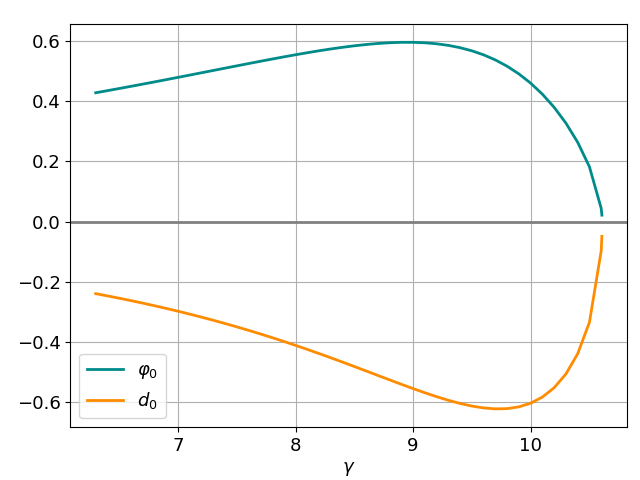
\includegraphics[scale=0.33]{oscillating_phi0d0_after_tangent_x0_045_beta_-1.png} \\ {\scriptsize a) $ \beta = -1.0 $}
\end{center}
\end{minipage} 
\hfill
\begin{minipage}[h]{0.49\linewidth}
\begin{center}
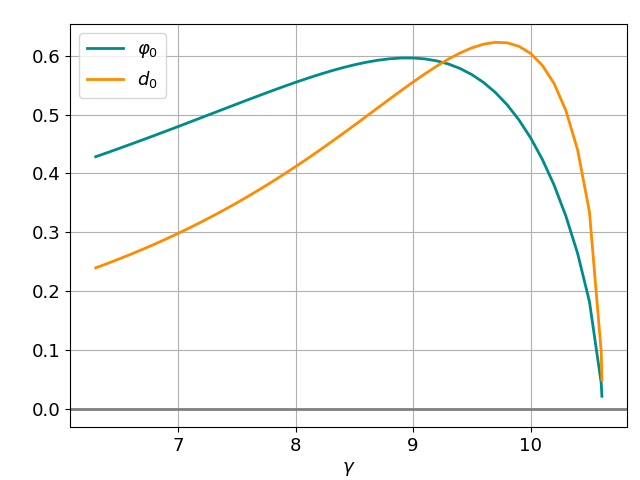
\includegraphics[scale=0.33]{oscillating_phi0d0_after_tangent_x0_045_beta_1.png}  \\ {\scriptsize b) $ \beta = 1.0 $}
\end{center}
\end{minipage} 
\end{figure}

$$ x_0 = 0.45 $$

\vfill

$$ \overline{\gamma} < \gamma < \Gamma_f. $$

\end{frame}

\begin{frame}

\begin{rustheorem}
Пусть $ \beta < 0 $, а $ \varepsilon = \alpha - \alpha_f $ для $ \overline{\gamma} \leqslant \gamma \leqslant \Gamma_f $, где $ \Gamma_f $ вычисляется с помощью \eqref{Gamma_f}. Тогда для любого $ \overline{\gamma} < \gamma < \Gamma_f $ существует $ \varepsilon_0 $ такое, что для $ \varepsilon \in (0, \varepsilon_0] $ система дифференциальных уравнений \eqref{problem_cube_in_cond}, \eqref{conditions_cube_in_cond} имеет в окрестности нуля орбитально инвариантный устойчивый цикл с асимптотикой \eqref{asymptotic_osc}.
\end{rustheorem}

\end{frame}

\end{document}